\begin{document}

\begin{document}

\chapter{Introdução}

A atual arquitetura de rede da Internet é composta por: nós (roteadores e switches, responsáveis pelo encaminhando de pacotes de dados) e os host(máquina de origem e destino de pacotes de dados, como computadores, servidores, smartphones, etc).Nesta arquitetura, os host fazem requisições entre si e realizam  troca de dados através de pacotes, utilizando diversos protocolos de acordo com a sua aplicação e os nós tem como função interligar o host com a rede para que o mesmo possa se comunicar.A transmissão de dados  é realizado pelos swtiches e roteadores da rede, que verificam o destino do pacote de dados e, utilizando uma tabela de encaminhamento, o redirecionam para o nós mais adequado ou para o seu destino final, como pode ser visto na figura \ref{Fig_Rede}.
\begin{figure}[h]
\centering
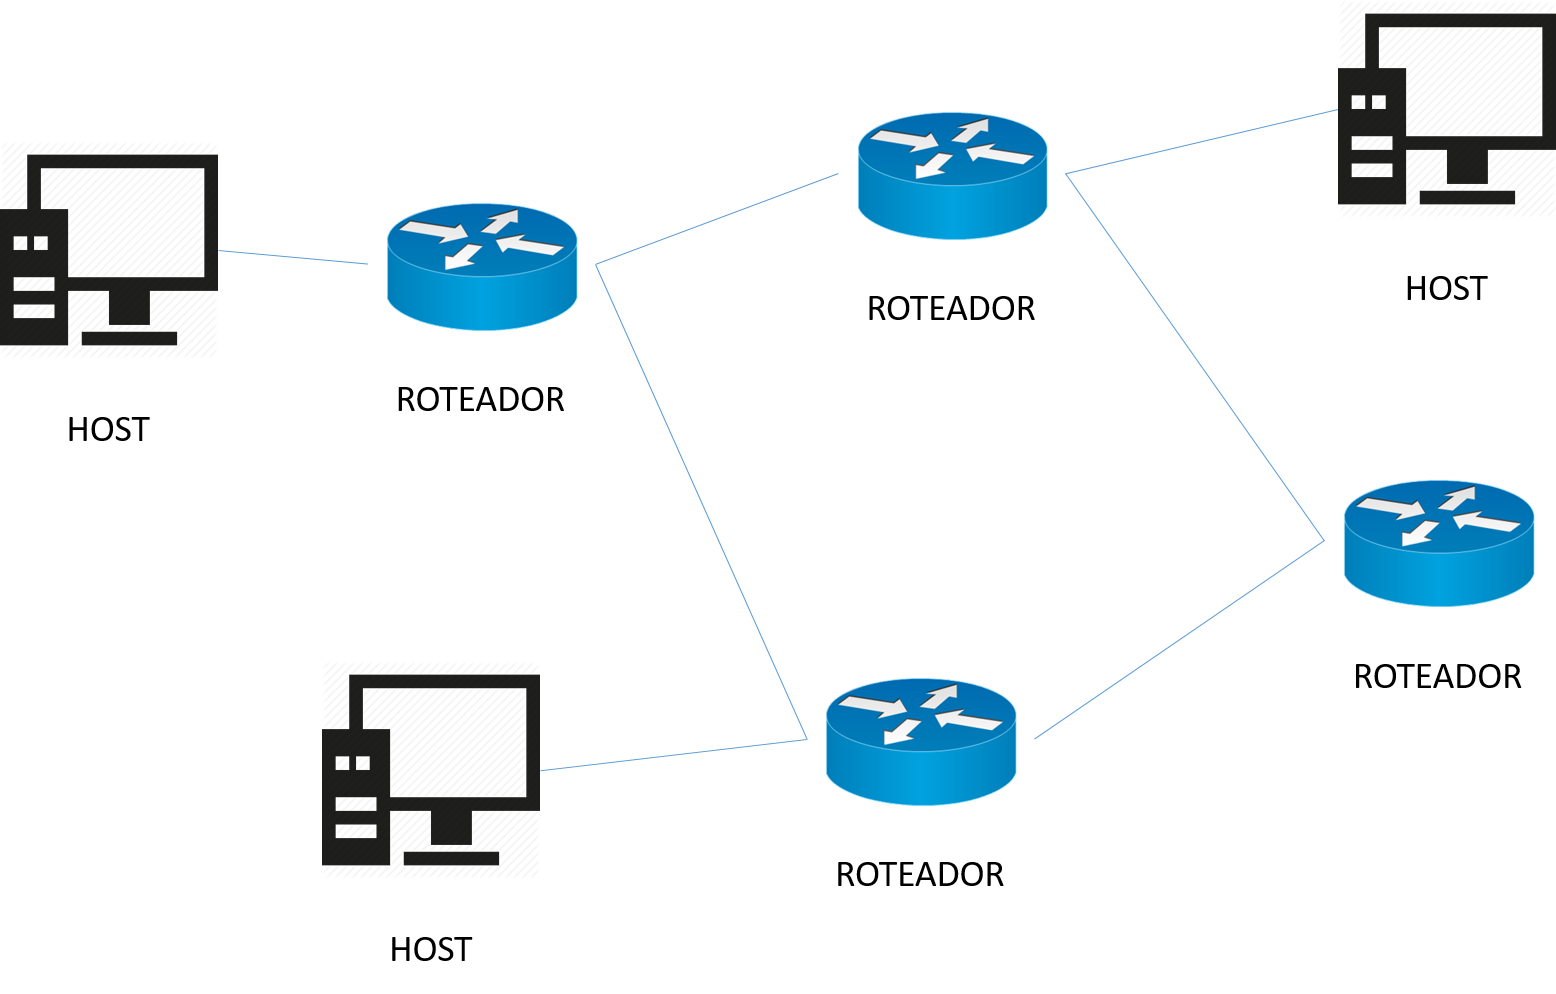
\includegraphics[width=0.7\textwidth]{Introducao/Rede.png}
\caption{Estrutura de uma Rede}
\label{Fig_Rede}
\end{figure}

Essa estrutura se mostrou extremamente eficiente, devido a sua escalabilidade e pela compatibilidade com diversos tipo de rede.Além disso, toda essa operação de consulta a tabela de encaminhamento e retransmissão de dados é realizada via hardware, aumentando a sua eficiência.

Apesar dessa estrutura reduzir o tempo de transmissão, e deixar os protocolos para as aplicações dentro dos host, ela também não fornece informações sobre a rede, dificultando o seu gerenciamento. Dessa forma, é difícil obter informações que ajudem a entender o estado em que a rede estava antes que ocorresse uma falha, além de desconhecer o tipo de trafego passa por ela.

Além disso, como a atual arquitetura é fortemente implementada via hardware,a implementação de novas tipos de arquitetura se torna custosa e pouco viável devido a necessidade de se trocar os diversos dispositivos já existentes, causando interrupções e instabilidade na rede ,sem contar nas falhas devido a falta de compatibilidade que podem ocorrer, inconvenientes pouco aceitáveis numa sociedade que se tornou extremamente dependente da Internet , que poderiam gerar grandes prejuízos financeiros para empresas dependentes destes serviços. Dessa forma, soluções baseadas em software se tornaram mais atraentes devido a possibilidade de serem implementadas sem troca de hardware e sem interrupção da rede. Uma dessas alternativas aqui apresentada é o paradigma SDN(Software Defined NetWork) juntamente com o protocolo OpenFlow.

No paradigma SDN, a tabela de encaminhamento utilizadas pelos  nós são definidas através de um software, e não mais por hardware, sendo assim, é possível organizar o trafego que passa pela rede em fluxos diferentes, e priorizá-los de acordo com a vontade do gerente da rede. Antes, cada dispositivo construía sua própria tabela de encaminhamento, possuindo apenas informações sobre os seus nós vizinhos. Já no paradigma SDN, todos os dispositivos são conectados a um dispositivo central, chamado de controlador, e ele, possuindo uma visão  completa da rede,se comunica com os nós através do protocolo Openflow e defini a tabela de encaminhamento de cada nó da rede.

Portanto, foi desenvolvida uma aplicação , utilizando linguagem de programação Python, capaz de monitorar e classificar o tipo de tráfego em uma placa de rede, e este trabalho tem como proposta a migração dessa aplicação para o controlador POX, para que o controlador possa fazer esse monitoramento e classificação de fluxo, de forma a melhor gerenciar a rede em caso de falha ou escassez de recurso da mesma.


\section{Objetivos}
\subsection{Objetivo geral}
O Objetivo deste trabalho é de criar um modulo no controlador POX de classificação e monitoramento de trafego de dados de uma rede usando a linguagem de programação Python, baseando-se em um módulo já existente.

\subsection{Objetivos Específicos}

\begin{itemize}
\item Criar um módulo de classificação no controlador POX
\item Classificar em 3 categorias o fluxo de dados: Netflix,Youtube,Outros
\item Armazenar as informações coletadas em um banco SQL para análise posterior
\item Verificar a resposta da rede após uma falha e verificar se a mesma consegue priorizar um tipo de fluxo em relação aos outros
\end{itemize}
\section{Estrutura do Trabalho}
Este trabalho é estruturado em 5 capítulos. No capítulo 2 serão explicados mais profundamente os conceitos de paradigma SDN, protoloco OpenFlow, Arquitetura de Rede,linguagem Pyhton, entre outros.A estrutura do novo módulo, especificações consideradas, funções e ferramentas utilizadas serão apresentados no capitulo 3, assim como o ambiente em que o módulo foi testado.


No capítulo 4 será feita uma exposição e análise dos resultados obtidos. E por fim, no capítulo 5 serão feitas as conclusões, considerações finais e trabalhos futuros.
\end{document}



\end{document}